\subsection{Degrees of freedom of the system}

CALIS has the capability to deploy sources at various positions inside the LSV. Besides the movement along z up to the maximum cable length, there is the possibility to articulate at an angle of $\theta$ between 90$^{\circ}$ and 180$^{\circ}$, where $\theta$ is the zenith-angle (Fig.~\ref{fig:coordinate_system}). Degrees between 0$^{\circ}$ and 90$^{\circ}$ are excluded because the end of the articulation chain is reached at an angle of 90$^{\circ}$ (see Fig.~\ref{fig:sourceArmRotation}).

\begin{figure}[htbp]
 \centering
  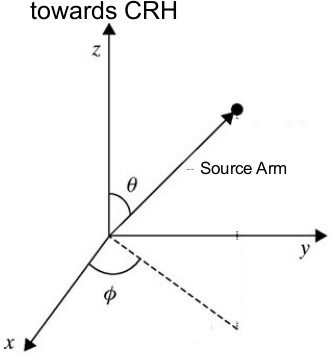
\includegraphics[width=0.4\textwidth]{Figures/coordinate_system}
  \caption{Spherical coordinate system used for establishing the direction of the rotation of CALIS-III and the articulation of the source arm. $\theta$ is kept at 90$^{\circ}$ when arm is articulated, and at 180$^{\circ}$ when dearticulated. $x$-axis is the direction toward the center of the detector. }
  \label{fig:coordinate_system}
\end{figure} 

\subsubsection{Rotation in the XY plane}\label{sec:XYrotation}
Below the view port is a sealed connection that has an o-ring seal and uses a ring clamp to compress the seal. The clamp can be slightly loosened to allow the assembly above and including the view port to be rotated with respect to the lower assembly and the detector. This rotation in the XY plane can even be performed while the gate valve is opened and the deployment device is deployed next to the cryostat, since the seal is helium leak and light tight even when loosened.

In principle a rotation in 360$\circ$ can be done, except when the arm would interfere with the cryostat. This has been used in one of the calibration campaigns to deploy a neutron source directly next to the cryostat and rotated away by 90$\circ$ in order to study optical shadowing effects from the cryostat (Sec.~\ref{sec:CalibCampaigns}). 

\mymarginpar{My impression is that a drawing to scale with the cryostat, the TPCthe organ pipe and the source arm would be good here}

For articulation, there is currently a choice of three arm lengths---40.31\,cm,  57.15\,cm and 62\,cm.  

Each of these lengths are measured from the center line of the organ pipe to the end of the source holder.  The arm lengths, 57.15\,cm and 62\,cm are intentionally made too long as they will be used to determine the exact location of the cryostat; some uncertainty in the cryostat's z and lateral position exist at the level of 3 - 4\,cm. The organ pipe we intend to use is 81\,cm distant from the cryostat center (and the geometric center of the LSV sphere) as measured from the center line of the organ pipe. The cryostat is 32\,cm in radius, which leaves a distance of $\sim$49\,cm to be reached  by the arm.


\begin{figure}[htbp]
 \centering
  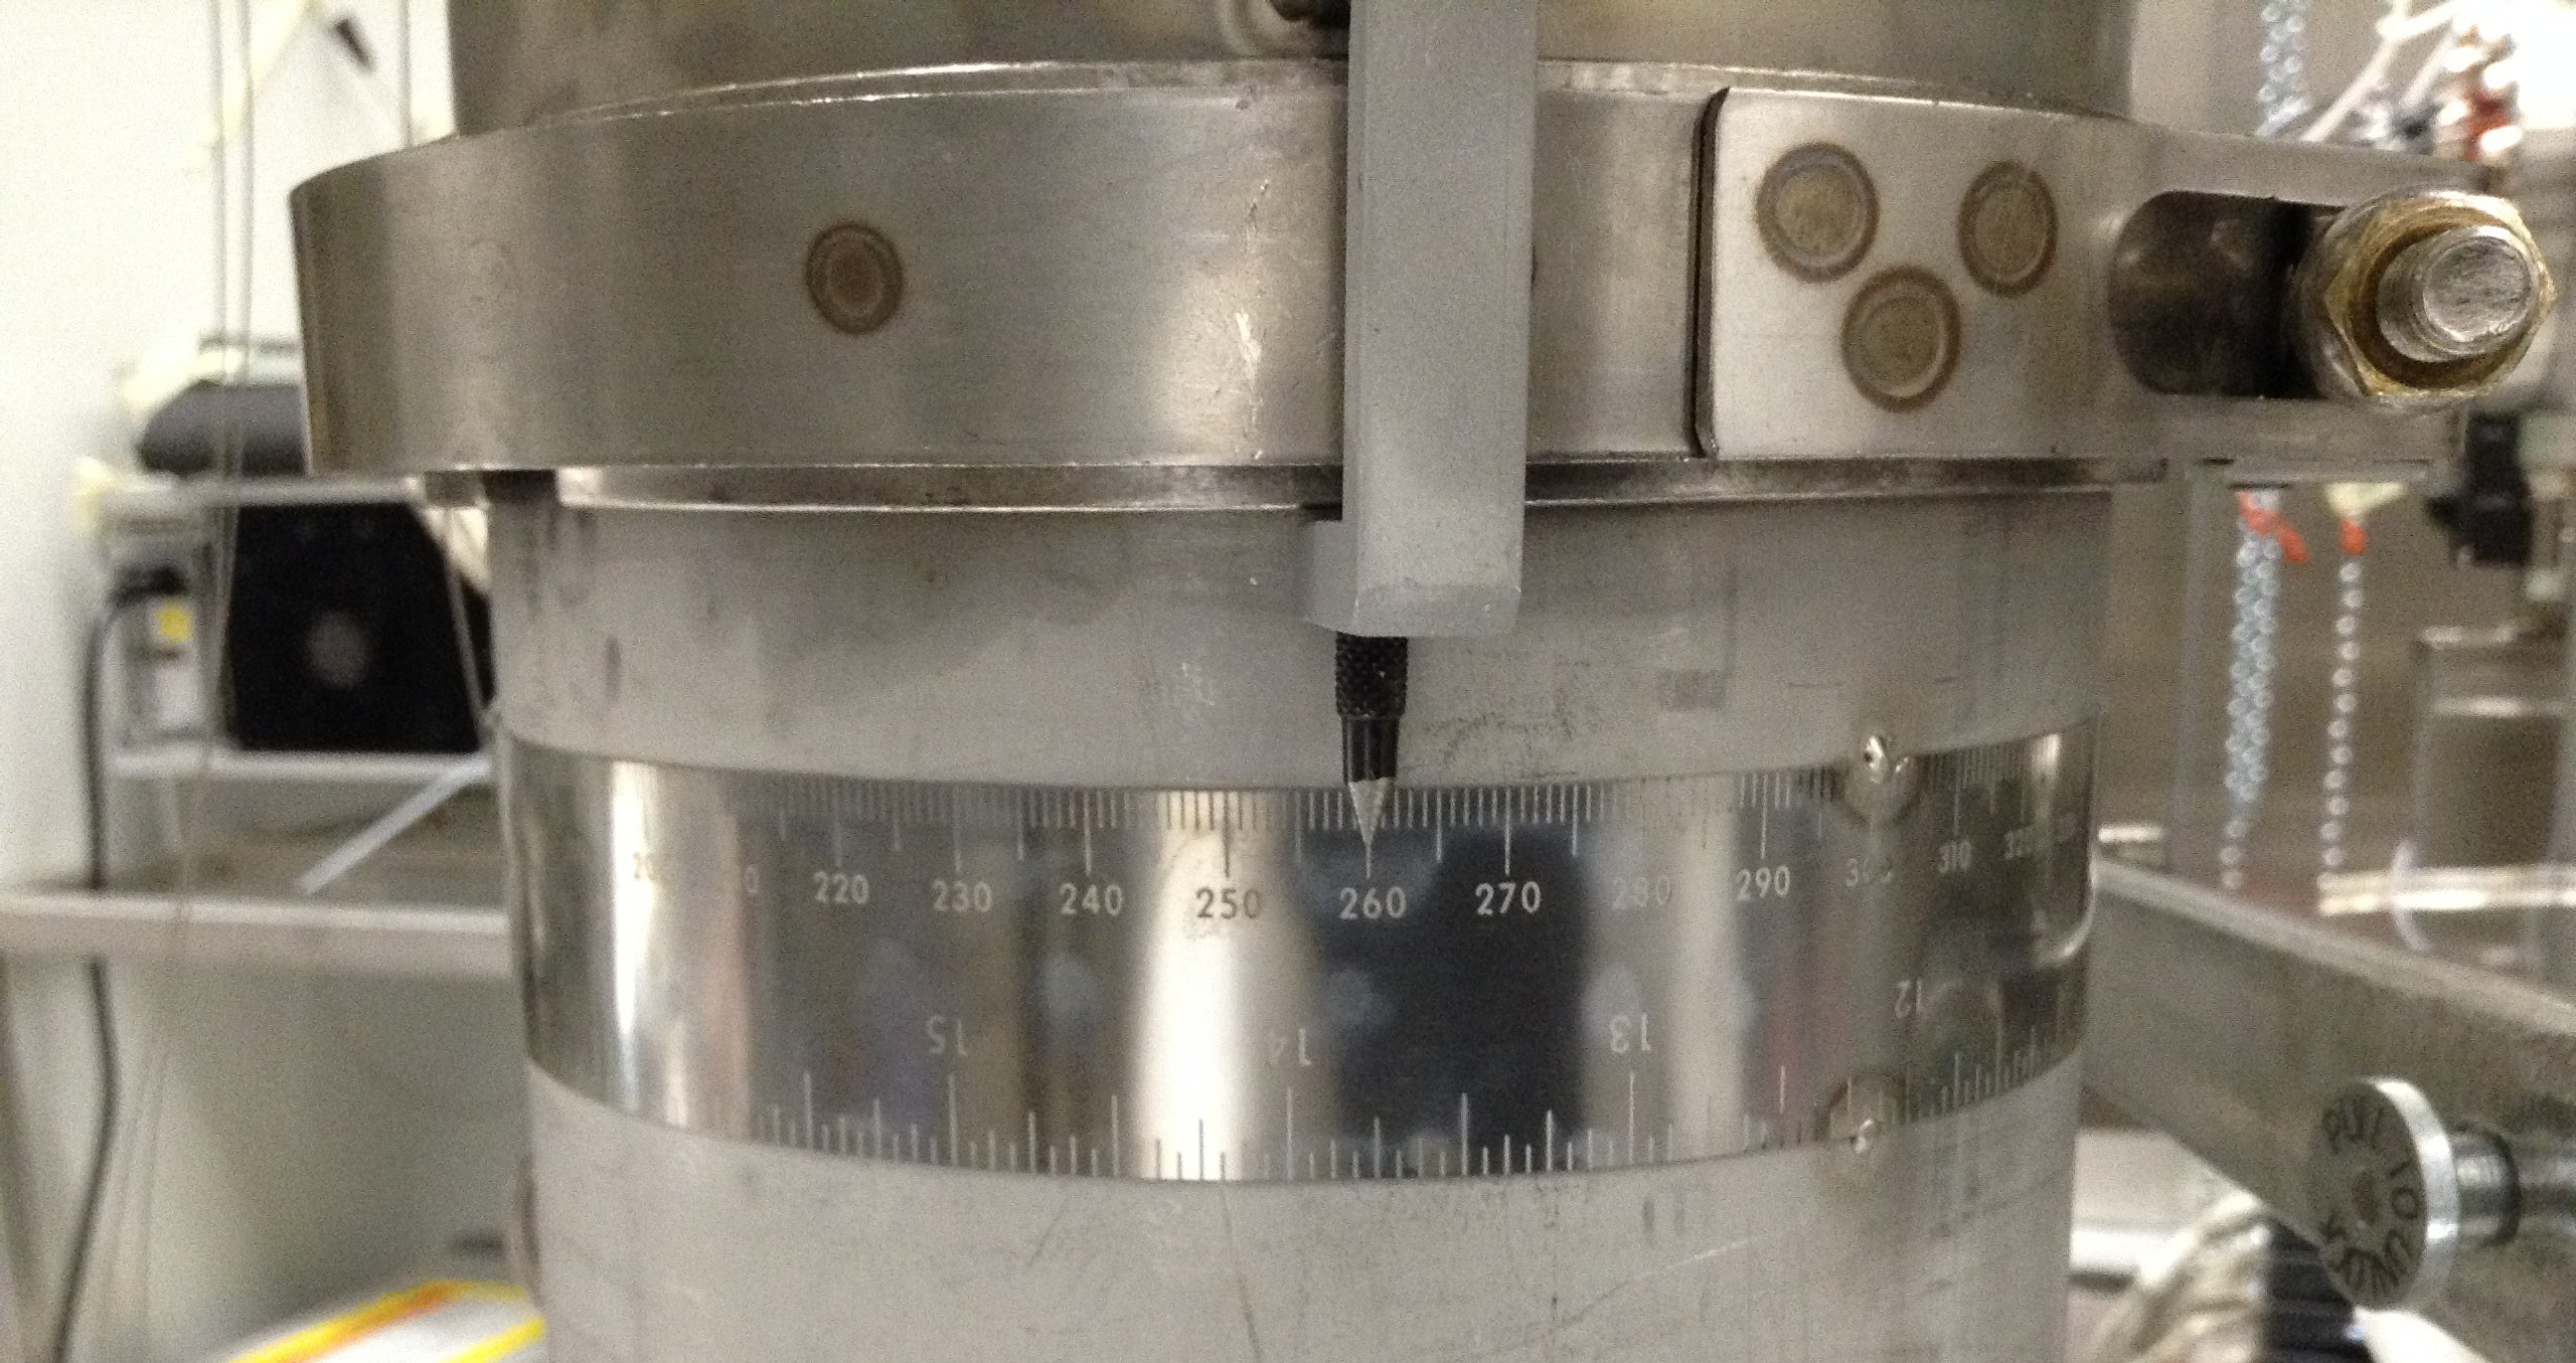
\includegraphics[width=0.7\textwidth]{Figures/RingClamp_WithPin_IMG_2669.JPG}
%  \includegraphics[scale=0.5]{Figures/RingClamp.jpg}
  \caption{Ring clamp  with the angle measuring strip shown below. In order to perform azimuthal rotation, the ring clamp is slightly loosened, and the entire upper assembly is rotated with respect to the lower assembly, along with the deployment device. The angle of rotation is read out from the strip that goes around the pipe. The strip is in mm, which has then been calibrated in degrees.}
  \label{fig:ring_clamp}
\end{figure} 

\subsubsection{``No fly'' zone}
Right above the cryostat where there are many supply tubes for the TPC a ``no fly'' zone has been defined. In this region no part of the deployment device may enter, in particular not the source arm.

\begin{figure}[htbp]
 \centering
  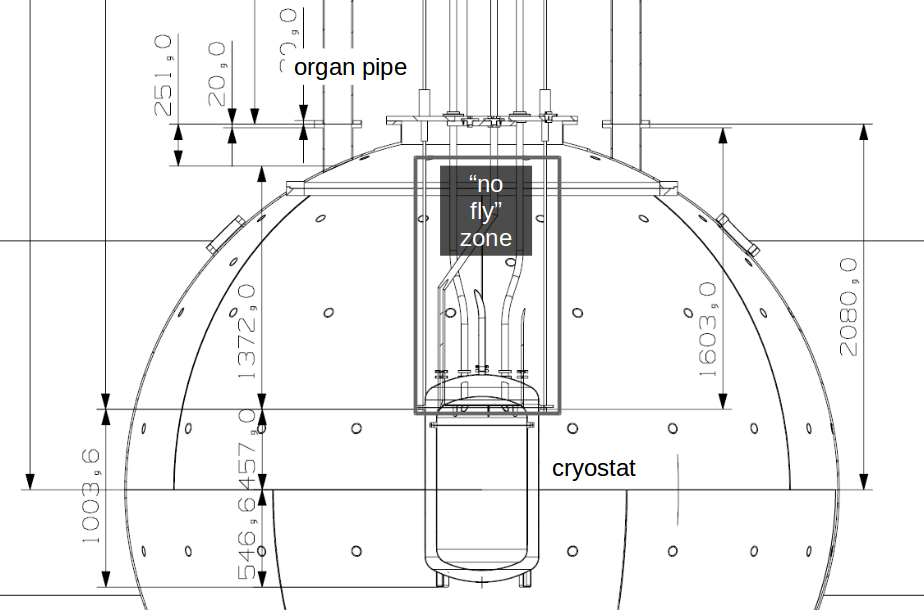
\includegraphics[scale=0.5]{Figures/NoFlyZone.png}
  \caption{``No fly'' zone for the CALIS source arm.}
  \label{fig:NoFlyZone}
\end{figure} 

\subsubsection{Default configuration}
By default the deployment device has been deployed with the longest arm (62 cm), at the center of the active volume of the TPC, with the arm rotated in the XY plane until contact with the cryostat has been made. Further details are provided in Sec.~\ref{sec:CalibCampaigns}.

Other degrees of freedom could involve shorter arm lengths, while longer arm lengths have been discussed but would require hardware modifications to the deployment device. Out of a total of four organ pipes a second one would be available for source calibration. A change in organ pipe would require a bigger effort involving also the crane in order to dismount CALIS and reinstall it on the other organ pipe. The remaining two pipes are too close to the cryo tower or reserved for the SABRE experiment \cite{SABRE}.

Finally CALIS is designed to house also a different deployment device, such as currently being planned for the neutron gun \cite{???}.